%!TEX root = paper.tex

\section{Context: The FAST Platform}
\label{sec:use_case}

The intention of this paper is to demonstrate the advances made regarding web service discovery and consumption through two artifacts developed as part of our research: the \emph{publishing and discovery platform} and the \emph{service wrapper tool}. While these artifacts may be deployed and used separately by third-party applications, they were originally developed to form the backbone of the FAST platform~\cite{hoyer2009fast}.
FAST constitutes a novel approach to application composition from a user-centric perspective. It is aimed at allowing users without previous programming experience to create their own situational applications by visually combining different \emph{building blocks}, such as graphical forms and back-end services, based on their inputs and outputs (or \emph{pre-} and \emph{post-conditions}). The work covered in this paper are the components highlighted in Fig.~\ref{fig:fast_architecture} by a dashed line. Communication within the platform is mostly done via a RESTful API, using JSON as an exchange syntax.
%These components have public interfaces to communicate with any application developed by a third-party developer or company, and as described in Sects. 3 and 4, are fully integrated and present a high cohesion with the rest of the components of the FAST architecture. 

\begin{figure}[ht]
  \begin{center}
    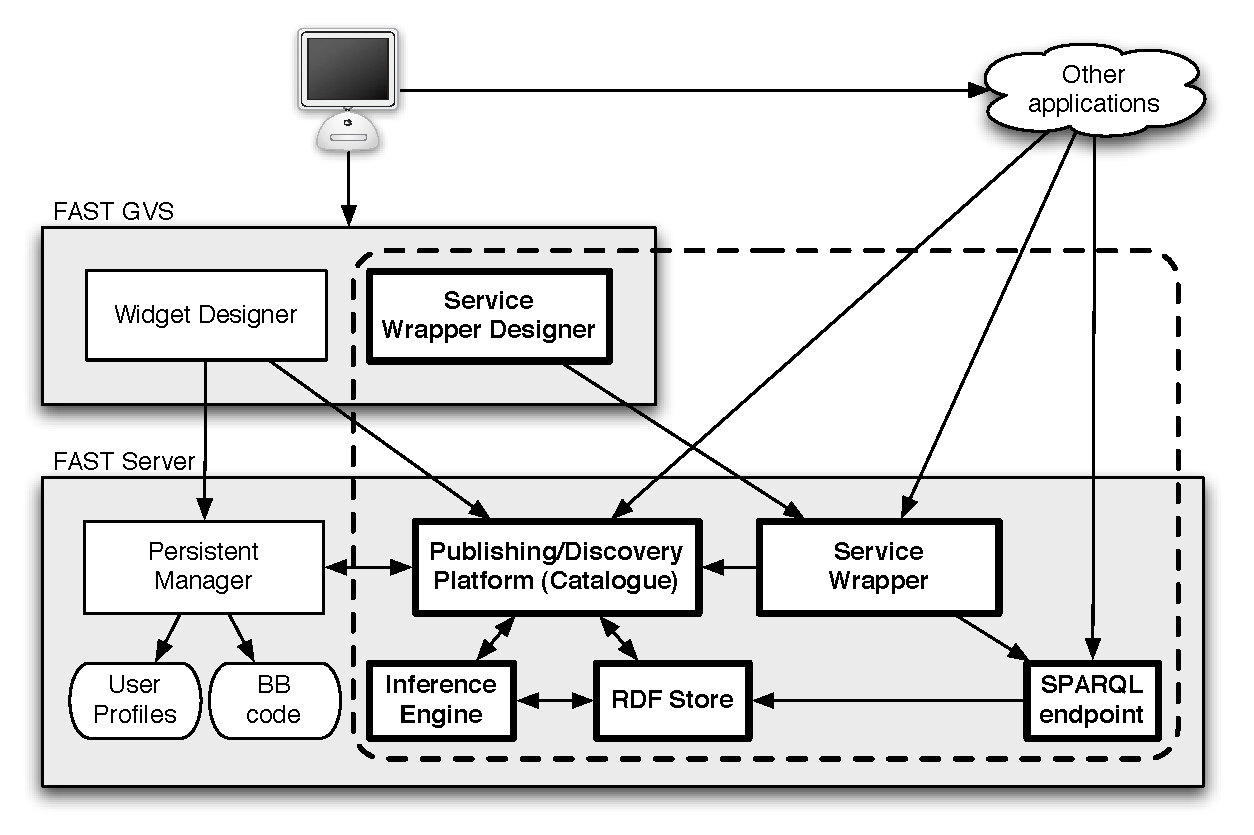
\includegraphics[width=\linewidth]{images/fast_architecture.pdf}
    \caption{Overview of the FAST architecture}
    \label{fig:fast_architecture}
  \end{center}
\end{figure}

In order to provide a better understanding of these components, we describe a number of concepts related to FAST in this section. 
A \emph{gadget} is the end product of the platform, ready to be run in any ordinary web browser, usually through a mashup platform. 
An undeployed gadget is also called \emph{screenflow}, which comprises a set of \emph{screens} connected through their \emph{pre-} and \emph{post-conditions}. A screen is the most complex building block fully functional by itself,
visually similar to a tab in a tabbed application.
It is composed by a \emph{form} conveying the graphical interface, and a set of \emph{operators} and \emph{back-end services}, wrapped into so-called \emph{service resources}.

The publishing platform, also called \emph{catalogue}, covers several important purposes, such as storage, indexing, publication and search of gadgets, gadget building blocks and user profiles.
% , as well as some level of ontology mediation to facilitate the integration of services from different parties (first steps in this direction are outlined in \cite{Ambrus:2009it}).
The service wrapper tool is used to create wrappers for third-party web services, transforming them into building blocks to be stored and reused within the FAST platform.
